% Created 2016-04-15 Fri 17:16
% Intended LaTeX compiler: pdflatex
\documentclass[11pt]{article}
\usepackage[utf8]{inputenc}
\usepackage[T1]{fontenc}
\usepackage{graphicx}
\usepackage{grffile}
\usepackage{longtable}
\usepackage{wrapfig}
\usepackage{rotating}
\usepackage[normalem]{ulem}
\usepackage{amsmath}
\usepackage{textcomp}
\usepackage{amssymb}
\usepackage{capt-of}
\usepackage{hyperref}
\usepackage{minted}
\usepackage[margin=0.75in]{geometry}
\newcommand{\norm}[1]{\Vert #1 \Vert}
\newcommand{\opnorm}[1]{\Vert #1 \Vert_{op}}
\newcommand{\fnorm}[1]{\Vert #1 \Vert_F}
\newcommand{\nucnorm}[1]{\Vert #1 \Vert_*}
\newcommand{\tr}{\operatorname{Tr}}
\newtheorem{theorem}{Theorem}[section]
\newtheorem{lemma}[theorem]{Lemma}
\newtheorem{proposition}[theorem]{Proposition}
\newtheorem{corollary}[theorem]{Corollary}
\newtheorem{proof}[theorem]{Proof}
\author{Bachir El khadir}
\date{\textit{<2016-04-02 Sat>}}
\title{Problem set 5, ORF523}
\hypersetup{
 pdfauthor={Bachir El khadir},
 pdftitle={Problem set 5, ORF523},
 pdfkeywords={},
 pdfsubject={},
 pdfcreator={Emacs 25.1.50.1 (Org mode )}, 
 pdflang={English}}
\begin{document}

\maketitle


\section{Problem 1}
\label{sec:orgheadline1}


Notation \(E_{ij} = (\delta_{ik}\delta_{jl} + \delta_{il}\delta_{jk})_{k,l}\) the matrix with all 0 except in \((i, j)\) and \((j, i)\)


\begin{align*}
-\nu(G) =
& \underset{X}{\text{min}}
& & Tr(X(-J)) \\
& \text{subject to}
& & X \ge 0
\\&&& Tr(XI_n) = 1 &(:& \alpha)
\\&&&Tr(E_{ij}X) = 0 \; \forall (i,j) \in E, i < j &(:& \lambda_{ij})
\end{align*}

has  for dual:

\begin{align*}
& \underset{\alpha, \lambda_{ij} \in \mathbb R}{\text{max}}
& & \alpha \\
& \text{subject to}
& & \alpha I + \sum_{(i,j) \in E, i < j} \lambda_{ij} E_{ij} \le -J
\end{align*}

Both are strictly feasible:
\begin{itemize}
\item for the primal, take \(X = \frac{I_n}n\)
\item For the dual, take \(\alpha = -2\), \(\lambda_{ij} = 0\)
\end{itemize}
Which proves that the dual and primal are equal. Taking  \(\beta = -\alpha\), we can write that as:



\begin{align*}
\nu(G) = 
& \underset{\alpha, \lambda_{ij} \in \mathbb R}{\text{min}}
& & \beta \\
& \text{subject to}
& & -\beta I + \sum_{(i,j) \in E, i < j} \lambda_{ij} E_{ij} \le -J
\end{align*}
Note that the \((1, 1)\) entry of \(-\beta I + \sum_{(i,j) \in E} \lambda_{ij} E_{ij} + J\): \(1-\beta\) shoud be negative, so we can ammend to the constraints that \(\beta \ge 1\)

\begin{align*}
-\beta I + \sum_{(i,j) \in E, i < j} \lambda_{ij} E_{ij} \le -J
&\iff \beta(I - \sum_{(i,j) \in E}, i < j \frac{\lambda_{ij}}{\beta} E_{ij}) \succeq J
\\&\iff I - \sum_{(i,j) \in E, i < j} \frac{\lambda_{ij}}{\beta} E_{ij}  \succeq \frac1\beta 11^T
\\&\iff \begin{pmatrix}I - \sum_{(i,j) \in E, i < j} \frac{\lambda_{ij}}{\beta} E_{ij} & \begin{matrix}1\\\vdots\\1\end{matrix}\\
 \begin{matrix}1&\ldots&1\end{matrix}&\beta\end{pmatrix}  \succeq 0 &\text{(By Schur Lemma bc $\beta > 0$)}
\end{align*}


Let's note this big matrix \(Z\). It is clear that a matrix \(Z \in S^{(n+1)}\) is of this form iff it verifies the constraints of the following optimization problem:
\begin{align*}
& \min
& & Z_{n+1, n+1} \\
& \text{subject to}
& & Z  \succeq 0
\\&&& Z_{i,n+1} = Z_{ii} = 1
\\&&& Z_{i,j} = 0 \forall \{i, j\} \in \bar E
\end{align*}

And this quantity is then equal to \(\vartheta(G)\).

Let's now prove the inequality (2).

Let \(C = \chi(\bar G)\).

By definition, there exist a partition of \(V\): \(\{V_1, \ldots, V_C\}\) such that \(V_i\) is a clique for all \(i \le C\)
\begin{itemize}
\item Define \(1_{V_i} \in \mathbb R^n\) to be the indicator function of the set \(V_i\), and note that \(1 = \sum_{i \le C} V_i\)
\item Define \(z_i = \begin{pmatrix}1_{V_i}\\1\end{pmatrix} \in \mathbb R^{n+1}\). Note that:
$$z_iz_i^T = \begin{pmatrix}1_{V_i}1_{V_i}^T&1_{V_i}\\1^T_{V_i}&1\end{pmatrix}$$
\item Define $$Z = \sum_{i} z_iz_i^T = \begin{pmatrix}\sum 1_{V_i}1_{V_i}^T&1\\1^T&C\end{pmatrix}$$
\(Z\) is positive semidefinite because it is a sum of psd terms \(z_iz_i^T\)
\item \((1_{V_i}1_{V_i}^T)_{kl} = (e_k^T1_{V_i})(e_l^T1_{V_i}) = 1_{V_i}(k) 1_{V_i}(l)\). If \((k, l) \in \bar E\), then the \(k^{th}\) node and the \(j^{th}\) node cannot be in the same \(V_i\), and therfore \((1_{V_i}1_{V_i}^T)_{kl} = 0\)
\item If \(k = l\), all the terms in \(\sum_i (1_{V_i}1_{V_i}^T)_{kl}\) are zero except for the \(i\) for which the \(k^{th}\) node is in \(V_i\), in which case it is equal to one.
\end{itemize}

As a conclusion, \(Z\) verifies all constraints of the dual, and \(Z_{n+1, n+1} = C = \chi(\bar G)\), so $$\chi(\bar G) \ge \vartheta(G)$$


\textbf{2}

Consider \(G = C_5\).

Using CVX to calculate \(\vartheta(G)\)
\begin{minted}[frame=lines,linenos=true]{matlab}
n = 5
J = ones(n, n);
cvx_begin sdp
variable X(n, n) symmetric;
maximize(trace(X*J))
X >= 0
X(5, 1) == 0
for i=1:4
    X(i, i+1) == 0
end
trace(X) == 1
cvx_end
ans=cvx_optval
\end{minted}

\begin{verbatim}
2.2361
\end{verbatim}


\(2 < \vartheta(G) < 3\)

\begin{itemize}
\item \(\vartheta(G) \not \in \mathbb N\)
\item \(\alpha(G), \chi(\bar G) \in \mathbb N\)

No inequality can thus be tight.
\end{itemize}

\section{Q2}
\label{sec:orgheadline4}

\textbf{1}


Consider 
\begin{align*}
\tag{P(G)}
& \min
& & Z_{n+1, n+1} \\
& \text{subject to}
& & Z \succeq 0
\\&&& Z_{i,n+1} = Z_{ii} = 1
\\&&& Z_{i,j} = 0 \forall \{i, j\} \in \bar E
\end{align*}


Write the lagrangian:


\begin{align*}
\mathcal L(Z, Y)
&= Z_{n+1, n+1} + \sum_{i=1}^n 2 Y_{i, n+1} (Z_{i, n+1} - 1) + Y_{ii} (Z_{ii} - 1) + \sum_{ij \in \bar E, i < j} Y_{ij}Z_{ij}
\\&= - \sum_{i} Y_{ii} + 2Y_{i, n+1} + \langle \underbrace{E_{n+1, n+1} + Y_{i, n+1} E_{i, n+1} + Y_{ii} E_{ii} + \sum_{ij \in \bar E, i < j}Y_{ij}E_{ij}}_{Y}, Z \rangle
\end{align*}

Dual:


\begin{align*}
\tag{$D_1(G)$}
& \max
& & \sum_{i \le n} - Y_{ii} - 2 Y_{i, n+1}\\
& \text{subject to}
& & Y \succeq 0
\\&&& Y_{n+1, n+1} = 1
\\&&& Y_{i,j} = 0 \forall \{i, j\} \in  E
\end{align*}

\(P(G)\) and \(D(G)\) are both strictly feasible (Consider \(I_{n+1}\) and \(E_{n+1, n+1}\) respectively). So theire optimal values are \textbf{attained and are equal}.

Let \(Y\) be a feasible solution, write:
\[Y = \begin{pmatrix}
&&&\\
&Y'&&y\\
&&&\\
&y^T&&1\end{pmatrix}\]

Note that by Schur's lemma:

$$Y \succeq 0 \iff Y' \succeq yy^T \iff Y' \succeq (-y)(-y)^T$$

So we can replace \(Y_{i, n+1}\) by \(-Y_{i, n+1}\) without affecting the optimal value:

\begin{align*}
\tag{$D_2(G)$}
& \max
& & \sum_{i \le n} - Y_{ii} + 2 Y_{i, n+1}\\
& \text{subject to}
& & Y \succeq 0
\\&&& Y_{n+1, n+1} = 1
\\&&& Y_{i,j} = 0 \forall \{i, j\} \in  E
\end{align*}


Let's now prove that this is equivalent to the following problem:


\begin{align*}
\tag{$D_3(G)$}
& \max
& & \sum_{i \le n}  Y_{ii} \\
& \text{subject to}
& & Y \succeq 0
\\& & &Y_{n+1, i} = Y_{ii} 
\\&&& Y_{n+1, n+1} = 1
\\&&& Y_{i,j} = 0 \forall \{i, j\} \in  E
\end{align*}

\begin{itemize}
\item If \(Y\) is feasible to \(D_3(G)\), then it is also feasible to \(D_2(G)\). Moreover in that case, \(\sum_{i} -Y_{ii} + 2Y_{i,n+1} =\sum_{i} Y_{ii}\), so \(D_2(G) \ge D_3(G)\)
\item Let \(Y\) be an optimal solution to \(D_2(G)\) (we proved that it exists), note \(\gamma = \sum_{i\le n} -Y_{ii} + 2 Y_{i, n+1} = D_2(G)\). Argue by contradiction that that \(Y_{n+1, j} - Y_{jj} \ne 0\).
\begin{itemize}
\item Note \(a = \sum_i Y_{ii} - 2Y_{i, n+1}\).

\item Note by \(Y'\) the matrix obtained from \(Y\) by multiplying the \(j^{th}\) row/column of \(Y\) by \(s \in \mathbb R\).
\item \(Y' = \operatorname{diag}(1 \ldots \underbrace{s}_j \ldots 1) Y  \operatorname{diag}(1 \ldots \underbrace{s}_j \ldots 1) \succeq 0\), and we can see that \(Y'\) is feasible in \(D_2(G)\).
\item Noting that \(Y'_{jj} = s^2 Y_{jj}, Y'_{j, n+1} = sY_{j, n+1}\), the objective value of \(Y'\) in \(D_2(G)\) is:
\end{itemize}
$$\sum_{i \le n} - Y'_{ii} + 2Y'_{i, n+1} - \gamma = - (s^2-1)  Y_{jj} + 2 (s-1) Y_{j, n+1} = -s^2 Y_{jj} + 2sY_{j, n+1} + Y_{jj}-2Y_{j, n+1}$$
The descriminant of the last equation in \(s\) is \(\Delta = 4[Y_{j, n+1}^2 + Y_{jj} (Y_{jj}-2Y_{j, n+1})] = 8Y_{j, n+1}(Y_{j, n+1} - Y_{j, n+1})\)
Note that by looking at a \(2 \times 2\) leading minor, \(Y_{jj} \ge Y_{n+1, j}^2\), and since \(Y_{jj} \ne Y_{n+1, j}\) they cannot be both equal to 0, so \(Y_{jj} > 0\). As a result, \(\Delta > 0\), meaning there exist an \(s\) that makes the objective value increase. 
Absurd.
\end{itemize}


We have that showed that \(Y\) verifies the satisfiability conditions of \(D_3(G)\), and therefore \(D_3(G) = \sum_{i} -Y_{ii} + 2Y_{i,n+1} =\sum_{i} Y_{ii} \le D_2(G)\)
Which completes the proof of the hint.


Let \(Y \in S^{n+1 \times n+1}\) be a feasible solution to this problem. Let \(x := (Y_{ii})_{i \le n}\). 

By consider the \(1 \times 1\) and \(2 \times 2\) minors:

\begin{align*}
Y \succeq 0 
&\implies \begin{vmatrix}Y_{ii}&Y_{ii}\\Y_{ii}&1\end{vmatrix} \ge 0, Y_{ii} \ge 0
\\&\implies Y_{ii} - Y_{ii}^2 \ge 0, Y_{ii} \ge 0
\\&\implies 0 \le Y_{ii}  \le 1
\end{align*}

We have just proved that \(0 \le x \le 1\)

Let \(\{i_1, \ldots, i_k\}\) a clique in the graph. Let \(I = \{i_1, \ldots, i_k, n+1\}\), and consider the principal minor:
\[\det Y_{I, I} = \det \begin{vmatrix}
Y_{i_1i_1} &    \ldots    &    0        & Y_{i_1i_1}\\
    0       & \ddots &   \vdots         & \vdots\\
    \vdots       &        & Y_{i_ki_k} & Y_{i_ki_k}\\
  Y_{i_1i_1}  &   \ldots     &  Y_{i_ki_k} & 1
\end{vmatrix} =
\det \begin{vmatrix}
x_{i_1} &    \ldots    &    0        & x_{i_1}\\
    0       & \ddots &   \vdots         & \vdots\\
    \vdots       &        & x_{i_k} & x_{i_k}\\
  x_{i_1}  &   \ldots     &  x_{i_k} & 1
\end{vmatrix}
\ge 0\]

To calculate this determinant, substract the sum of the first \(n\) rows from the last one to get a triangular matrix:
\[\det Y_{I, I} = \det \begin{vmatrix}
x_{i_1} &    \ldots    &    0        & x_{i_1}\\
    0       & \ddots &   \vdots         & \vdots\\
    \vdots       &        & x_{i_k} & x_{i_k}\\
  0  &   \ldots     &  0 & 1 - x_{i_1} - \ldots x_{i_k}
\end{vmatrix} = x_{i_1} \ldots x_{i_k} (1 - x_{i_1} - \ldots -x_{i_k}) \]

Which means that \(x_{i_1} + \ldots + x_{i_k} \le 1\), eg \(x\) respects all the clique inequalities.


As a result:
$$\sum_{i=1}^n Y_{ii} = \sum_{i=1}^n x_i \le \eta^{(k)}_{LP}$$

Taking the sup over feasible \(Y\):
\(\vartheta(G) \le \eta_{LP}^{(k)}\)



\textbf{2}
\begin{org}
\begin{center}
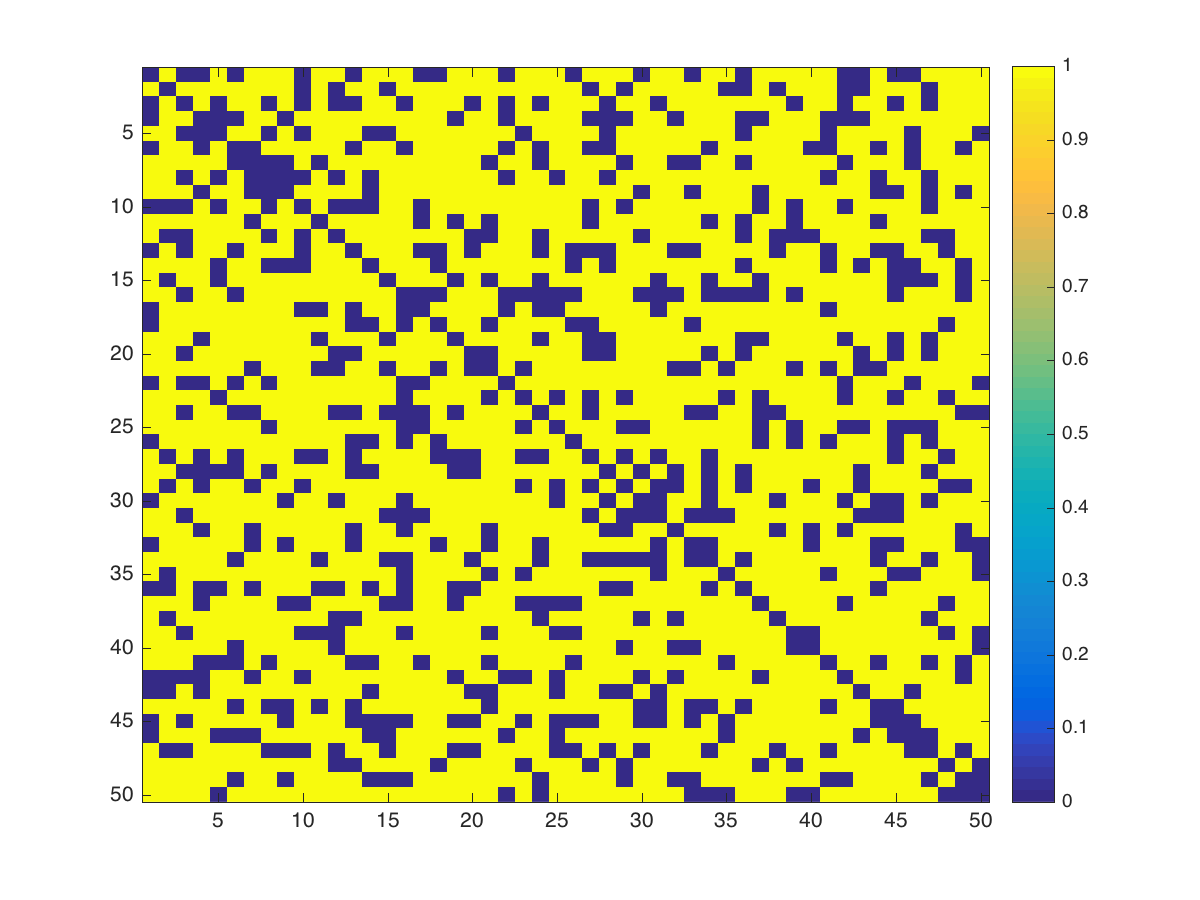
\includegraphics[width=0.35\textwidth]{graph.png}
\captionof{figure}{G Adjacency matrix}
\end{center}
\end{org}




\subsection{\(\vartheta(G)\)}
\label{sec:orgheadline2}
\begin{minted}[frame=lines,linenos=true]{matlab}
n = 50
J = ones(n, n);

cvx_begin sdp
variable X(n, n) symmetric;
maximize(trace(X*J))
X >= 0
for i=1:n
    for j=1:i
        if G(i, j) == 1
            X(i, j) == 0
        end
    end
end
trace(X) == 1
cvx_end

ans=cvx_optval
\end{minted}

\begin{verbatim}
5
\end{verbatim}


\begin{org}
\begin{center}
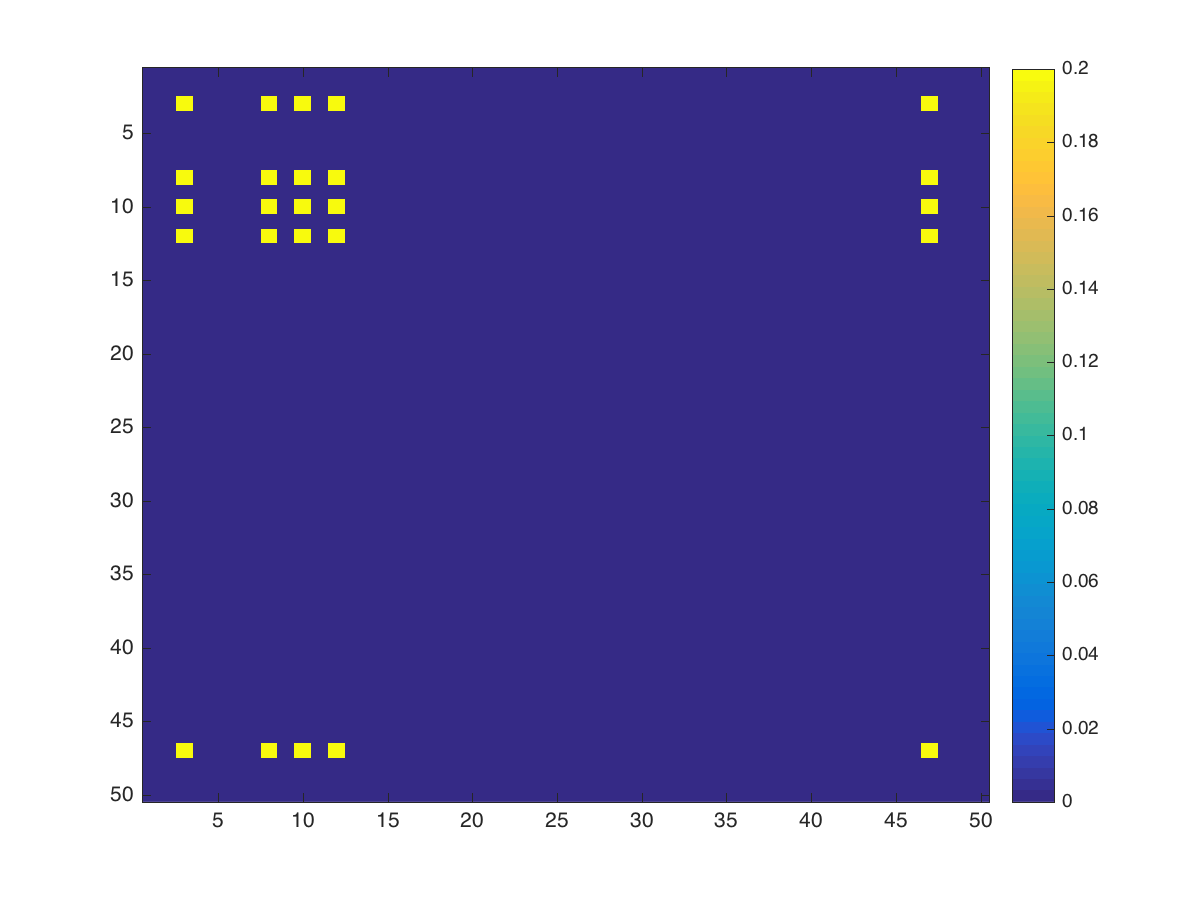
\includegraphics[width=0.35\textwidth]{X.png}
\captionof{figure}{X optimal solution}
\end{center}
\end{org}





Note that the resulting \(X\) is of rank 1, so it can be decomposed into \(X = xx^T\). We check that \(V_x = \{i , x_i \ne 0\}\) represents indeed a stable set.
\begin{minted}[frame=lines,linenos=true]{matlab}
[v,e] = eigs(full(X),1);
stableset = find(abs(v) > 0.01)  
ans=stableset'
\end{minted}

\begin{center}
\begin{tabular}{rrrrr}
3 & 8 & 10 & 12 & 47\\
\end{tabular}
\end{center}


\begin{minted}[frame=lines,linenos=true]{matlab}
G(stableset, stableset)
\end{minted}

\begin{org}
\begin{center}
\captionof{table}{Subgraph of the nodes in the stableset}
\begin{tabular}{rrrrr}
0 & 0 & 0 & 0 & 0\\
0 & 0 & 0 & 0 & 0\\
0 & 0 & 0 & 0 & 0\\
0 & 0 & 0 & 0 & 0\\
0 & 0 & 0 & 0 & 0\\
\end{tabular}
\end{center}
\end{org}


Let's assume that there exist another stable set of size 5.

This would mean that there exist \(v \in V_x\) such that imposing \(x_j = 0\) (eg \(X_{jj} =  0\)) would not change \(\alpha\). Let's check:

\begin{minted}[frame=lines,linenos=true]{matlab}
  n = 50
  J = ones(n, n);
  opt = [stableset, zeros(5, 1)]
  for vi=1:5
      v = stableset(vi)
      cvx_begin sdp
      variable Y(n, n) symmetric;
      variable optvalue;
      maximize(trace(Y*J))
      Y >= 0
      for i=1:n
          for j=1:i
              if G(i, j) == 1
                  Y(i, j) == 0
              end
          end
      end
      Y(v,v) == 0
      trace(Y) == 1
      optvalue == trace(Y*J)
      cvx_end
      opt(vi, 2) = optvalue
  end
ans=opt
\end{minted}

\begin{org}
\begin{center}
\captionof{table}{Lovazs}
\begin{tabular}{rr}
Node removed & Lovasz of the subgraph\\
\hline
3 & 4.4463\\
8 & 4.5191\\
10 & 4.512\\
12 & 4.5586\\
47 & 4.4771\\
\end{tabular}
\end{center}
\end{org}



Since Lovasz number \(\vartheta\) is an upper bound on \(\alpha\), This proves that any stable set not containing one of the nodes in \(V_x\) is of size less than \(5\).

We have just proved uniqueness of the stable set.

\subsection{\(\mu^{LP}\)}
\label{sec:orgheadline3}

k = 2

\begin{minted}[frame=lines,linenos=true]{matlab}
cvx_begin 
variable x(n)
maximize(sum(x))
for i=2:n
    for j=1:(i-1)
        if G(i, j) == 1
            x(i) + x(j) \langle = 1
        end
    end
end
0 <= x <= 1
cvx_end

ans=cvx_optval
\end{minted}

\begin{verbatim}
50
\end{verbatim}


k = 3

\begin{minted}[frame=lines,linenos=true]{matlab}
cvx_begin 
variable x(n)
maximize(sum(x))
for i=2:n
    for j=1:(i-1)
        if G(i, j) == 1
            x(i) + x(j) <= 1
        end
        for r=1:(j-1)
            if G(i, j) +  G(j, r) + G(r, i) == 3
                x(i) + x(j) + x(r) <= 1
            end
        end
    end
end
0 <= x <= 1
cvx_end

ans=cvx_optval
\end{minted}

\begin{verbatim}
16.667
\end{verbatim}

k = 4
\begin{minted}[frame=lines,linenos=true]{matlab}
M = 50
cvx_begin 
  variable x(n)
  maximize(sum(x))
  for i=2:M
      for j=1:(i-1)
          if G(i, j) == 0
              continue
          end
          x(i) + x(j) <= 1
          for r=1:(j-1)
              if G(j, r) == 0 || G(r, i) == 0
                  continue
              end
              x(i) + x(j) + x(r) <= 1
              for p =1:(r-1)
                  if G(i, p) == 0 || G(j, p) == 0 || G(r, p) == 0
                      continue
                  end
                  x(i) + x(j) + x(r) + x(p) <= 1
              end
          end
      end
  end
  0 <= x <= 1
  cvx_end

  ans=cvx_optval
\end{minted}

\begin{verbatim}
12.5
\end{verbatim}


\section{Problem 3}
\label{sec:orgheadline5}
\textbf{1.}
Let \((a, b), (u, v)\) be two nodes in \(G_A \otimes G_B\)
The two nodes are connected if and only if:
\begin{itemize}
\item \(A_{au} = 1, A_{bv} = 1\)
\item \(a = u, A_{bv} = 1\)
\item \(A_{au} = 1, b = v\)
\end{itemize}
This can be summerised as \((A_{au} + \delta_{au})(A_{bv} + \delta_{bv}) - \delta_{au}\delta_{bv} = 1\)

So the adjacency matrix of \(G_A \otimes G_B\) is
\((A+I_{n}) \otimes (B+I_m) - I_{nm}\).

Where \(\otimes\) denote the Kronecker product: \((A\otimes B)_{p(r-1)+v, q(s-1)+w} = A_{rs} B_{vw}\)

\textbf{2.}

$$5 = \alpha(G) \le \Theta(G) \le \vartheta(G) = 5$$
so \(\Theta(G) = 5\)



\section{Problem 4}
\label{sec:orgheadline6}

\textbf{1.}
(1) is equivalent to
\[\left\{\begin{array}{cc}
  x^TAy &= \max_{\tilde x \in \Delta_m} \tilde x^TAy\\
  x^TBy &= \max_{\tilde y \in \Delta_n}  x^TB\tilde y
  \end{array}\right.\]

Consider the first problem:
$$\max_{\tilde x \in \Delta_m} \tilde x^TAy$$

This is an LP whose feasible region   \(\Delta_m = conv(e_i, i=1\ldots m)\) is compact, so the maximum is attained in one of the extreme points \(e_{i_0}\). Therefore 

$$x^TAy = \max_{\tilde x \in \Delta_m} \tilde x^TAy \iff x^TAy = e_{i_0}^TAy = \max_{i} e_i^TAy \iff x^TAy \ge e_i^TAy \forall i$$
Same argument applies for \(y\) so that:
$$x^TBy = \max_{\tilde y \in \Delta_n} x^TB \tilde y  \iff x^TAy \ge x^TBe_i \forall i$$

So: \[(1) \iff \left\{\begin{array}{cc}
  x^TAy &\ge e_i^TAy \; \forall i = 1\ldots m\\
  x^TBy &\ge x^TAe_i \; \forall i = 1\ldots n
  \end{array}\right.\]

\textbf{2.}

\(x \in \Delta_m, y \in \Delta_n\)

Note \(z = \begin{pmatrix}x \\ y\\1\end{pmatrix}, u = \begin{pmatrix}1 \\ 0\end{pmatrix}, v = \begin{pmatrix}0 \\ 1\end{pmatrix}\), 
\[M = zz^T = \begin{pmatrix}xx^T&xy^T&x\\yx^T&yy^T&y\\x^T&y^T&1\end{pmatrix}\]

Note that
\begin{itemize}
\item \(M \succeq 0\)
\item \(rank(M) = 1\)
\item \(M_{n+m:n+m+1, 1:n} = x \in \Delta_n\)
\item \(M_{n+m:n+m+1, n+1:n+m} = y \in \Delta_m\)
\item \(M_{n+m+1, n+m+1} = 1\)
\end{itemize}

Now to express the fact that \((x, y)\) is a Nash equilibrium (*):
\begin{itemize}
\item \(tr(M_{n+1:n+m, 1:n} A) = tr(yx^T A) = tr(x^TAy) \ge tr(e_i^TAy) \ge tr(e_i^TAM_{n+m:n+m+1, n+1:n+m})\)
\item \(tr(M_{n+1:n+m, 1:n} B)  \ge tr(M_{n+m:n+m+1, 1:n}Ae_i)\)
\end{itemize}

Now let \(M \in S^{n+m}\), verifying all the previous conditions. Then by cholesky, there existe a vector \(z \in \mathbb R^{n+m+1}\), such that: \(M = zz^T\)

\begin{itemize}
\item Let's decompose \(z := \begin{pmatrix}x \\ y\\\alpha\end{pmatrix} \in \mathbb R^{n+m+1}\), so that \(M = zz^T = \begin{pmatrix}xx^T&xy^T&\alpha x\\yx^T&yy^T&\alpha y\\\alpha x^T&\alpha y^T&\alpha^2\end{pmatrix}\)
\item \(1 = M_{n+m+1, n+m+1} = \alpha^2 \implies \alpha=\pm 1\)
\item \(M_{n+m:n+m+1, 1:n} = \alpha x \in \Delta_n\)
\item Similarly: \(\alpha y \in \Delta_m\)
\item If \(\alpha = -1\), we can always change \(z\) to \(-z\) without loss of generality to make \(x, y \ge 0\) and therefore \(x \in \Delta_m, y \in \Delta_n\)
\item \((x, y)\) naturally represent a Nash equilibrium due to (*).
\end{itemize}

PSD relaxation:
\begin{itemize}
\item \(M \succeq 0\)
\item \(M_{n+m:n+m+1, 1:n} \in \Delta_n\)
\item \(M_{n+m:n+m+1, n+1:n+m} \in \Delta_m\)
\item \(M_{n+m+1, n+m+1} = 1\)
\end{itemize}

Moreover, we can add the following constraints:

\begin{itemize}
\item The sum of the columns of \(M_{1:n, 1:n} = xx^T = (x_ix_j)_{ij}\) is equal to \(x\). (This is true because \(x \in \Delta_n\))
\item Similarly the sum of the columns of \(M_{n+1:n+m, n+1:n+m}\) is equal to \(y\).
\item The sum of the columns of \(M_{n+1:2n, 1:n} = yx^T\) is equal to \(y\), and the sum of the rows is equal to \(x\).
\item \(M \ge 0\)
\end{itemize}

\begin{minted}[frame=lines,linenos=true]{matlab}
A = [345 78 97 355 264 528;
     310 52 483 385 541 276;
     236 248 445 243 7 80;
     64 23 290 226 157 426;
     292 129 300 116 628 580;
     477 317 342 58 152 106]

B = [404 183 215 531 232 31;
     79 624 442 145 277 182;
     421 619 1 271 477 456;
     561 364 423 539 96 147;
     632 546 528 580 388 229;
     279 112 198 97 172 94]

n = length(A)
In = eye(n, n);

cvx_begin sdp
variable M(2*n+1, 2*n+1) symmetric;
variables x(n) y(n);
variables yx(n, n) xx(n, n) yy(n, n);

maximize(trace(yx * A))

M >= 0
M(2*n+1, 2*n+1) == 1
for i=1:(2*n+1)  
    for j=1:(2*n+1)
        M(i, j) >= 0
    end  
end

% sub-blocks of M
x == M(1:n, 2*n+1)
y == M(n + (1:n), 2*n+1)
xx == M(1:n, 1:n)
yy == M(n + (1:n), n + (1:n))
yx == M(n + (1:n), 1:n)

% x and y in the simplex
sum(x) == 1
sum(y) == 1

% Additional constraints
x == sum(xx)'
y == sum(yy)'
x == sum(yx')'
y == sum(yx)'

% Nash equilibrium constraint
for i=1:n
    ei = In(1:n, i);
    trace(yx * A) >= trace(ei' * A * y)
    trace(yx * B) >= trace(x' * B * ei)
end

cvx_end

ans=cvx_optval;
\end{minted}

\begin{verbatim}
443.13
\end{verbatim}





Which proves that the score of the first player cannot exceed \(434\)
\end{document}